Nesse capítulo, serão apresentados os resultados obtidos utilizando o método multiescala para solução dos sistemas lineares decorrentes do operador apresentado no capítulo \ref{ch:modelagem}. Os resultados são apresentados na seguinte ordem: resultados em casos que a solução analítica é conhecida para testar o bom funcionamento do método e comparações do método multiescala como pré-condicionador contra solver multigrid.


\begin{table}[]
\caption{Tabela com os casos que serão apresentados os resultados}
\centering
\begin{tabular}{ccccl}
\cline{1-4}
\multicolumn{1}{|c|}{\textbf{Nome}} & \multicolumn{1}{c|}{\textbf{Nx}} & \multicolumn{1}{c|}{\textbf{Ny}} & \multicolumn{1}{c|}{\textbf{Caso Real}} &  \\ \cline{1-4}
\multicolumn{1}{|c|}{caso A}        & \multicolumn{1}{c|}{100}         & \multicolumn{1}{c|}{100}         & \multicolumn{1}{c|}{}                   &  \\ \cline{1-4}
\multicolumn{1}{|c|}{caso B}        & \multicolumn{1}{c|}{320}         & \multicolumn{1}{c|}{320}         & \multicolumn{1}{c|}{}                   &  \\ \cline{1-4}
\multicolumn{1}{|c|}{caso C}        & \multicolumn{1}{c|}{103}         & \multicolumn{1}{c|}{56}          & \multicolumn{1}{c|}{}                   &  \\ \cline{1-4}
\multicolumn{1}{|c|}{caso D}        & \multicolumn{1}{c|}{244}            & \multicolumn{1}{c|}{71}            & \multicolumn{1}{c|}{Sim}                &  \\ \cline{1-4}
\multicolumn{1}{|c|}{caso  E}       & \multicolumn{1}{c|}{582}         & \multicolumn{1}{c|}{336}         & \multicolumn{1}{c|}{Sim}                &  \\ \cline{1-4}
\multicolumn{1}{l}{}                & \multicolumn{1}{l}{}             & \multicolumn{1}{l}{}             & \multicolumn{1}{l}{}                    &  \\
\multicolumn{1}{l}{}                & \multicolumn{1}{l}{}             & \multicolumn{1}{l}{}             & \multicolumn{1}{l}{}                    & 
\end{tabular}
\end{table}


\section{Soluções Analíticas}

Inicialmente, é necessário atestar que o código de elementos finitos está resolvendo corretamente o operador da equação \ref{eq:edp_geomec}. 
Para isso, foi montado teste semelhante ao mostrado em \cite{irina}, teste consiste em encontrar solução para o problema que possui solução analítica de acordo com a equação mostrada em \ref{eq:irinasol} 
em um domínio $L \times W$.


\begin{equation} \label{eq:irinasol}
  \begin{aligned}
  u_x = 10^{-5} sen(\frac{\pi x}{L}) sen(\frac{\pi y}{W})  \\
  u_y = 10^{-5} sen(\frac{\pi (L-x)}{L}) sen(\frac{\pi x}{W})
  \end{aligned}
\end{equation}

Dada essa solução, é possível calcular o operador do lado direito aplicando o operador e obtendo a função $f: R^2 \rightarrow R^2$ apresentada em \ref{eq:irinald}

\begin{equation} \label{eq:irinald}
f(x, y) = 
\left[\begin{matrix}\frac{E \left(- 2 v + \pi^{2} y \left(v - 1\right) \left(y - 2\right) + 1\right) \sin{\left (\pi x \right )}}{\left(v + 1\right) \left(2 v - 1\right)} \\ \frac{\pi E \left(y - 1\right) \cos{\left (\pi x \right )}}{\left(v + 1\right) \left(2 v - 1\right)}\end{matrix}\right]
\end{equation}

Dessa forma, as equações que representam o problema resolvido são apresentadas em \ref{eq:irinaproblem}
\begin{equation}\label{eq:irinaproblem}
    \begin{aligned}
        S^T C S u = f(x, y) \\
        u(x,y) = [0, 0]^T, \text{ em } \Gamma \\
        L = W = 10
    \end{aligned}
\end{equation}


O erro entre a solução calculada pelo método dos elementos finitos pode então ser comparada
com a solução analítica pode ser calculado conforme a equação 

\begin{equation} \label{eq:erroAnalitico}
    \epsilon_{inf} =\frac{|u_{fem} - u_{analitico}|}{|u_{analitico}|}
\end{equation}

onde $u_{analitico} = [u_x(x_0, y_0), u_y(x_1, y_1), ..., u_x(x_{n_n}, y_{n_n})] ^ T$ e $u_{fem}$ é a solucão obtida com o método dos elementos finitos. Esse erro é mostrado na \ref{fig:SecondOrderTest} onde no eixo x 
está plotado no eixo x o logaritmo do tamanho de cada elemento e no eixo y o logaritmo do erro analítico também mostra uma reta de coeficiente angular $2$ para comparação com um decaimento
quadrático do erro em função do tamanho de cada elemento da malha.

\begin{figure}[!htbp]
    \label{fig:SecondOrderTest}
    \centering
    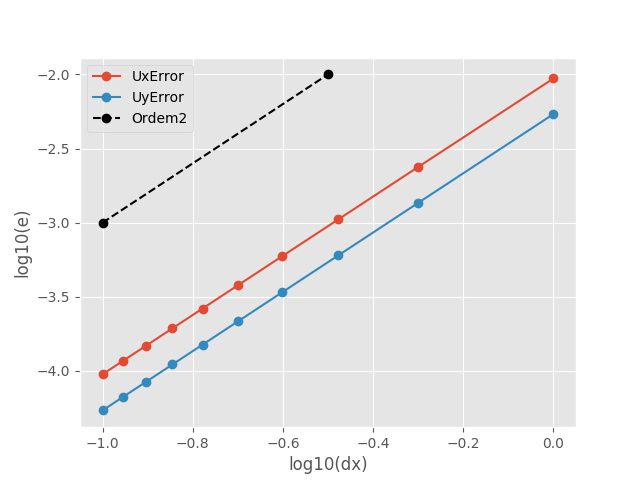
\includegraphics[width=7cm]{chap08/figs/SecondErrorTest.png}
    \caption{Comparação entre solução do grid fino e de diferentes grids grossos.}
\end{figure}
    
Um segundo caso com resultado analítico é a condição de cisalhamento puro (Simple Shear). 
Nesse caso, o problema é definido na forma apresentada em \ref{eq:simpleshear}. A solução
é dada por $u(x,y) = [0, y]^T$. Portanto, dado que o a solução é um polinomio do primeiro grau,
essa pode ser representada pelo espaço gerado pelas funções de base bilineares e, então,
os erros de truncamento nesse caso não existem ficando apenas com erros de arredondamento.

\begin{equation}\label{eq:simpleshear}
    \begin{aligned}
        S^T C S u = 0 \\
        u(x,y) = [10^{-6}, 0]^T, \text{ em } {x, y \in \Gamma | y \neq 1} \\
        u(x,y) = [10^{-6}y, 0]^T, \text{ em } {x, y \in \Gamma | x = 0 \text{ ou } x = 1} \\
        u(x,y) = [0, 0]^T, \text{ em } y=0
    \end{aligned}
\end{equation}

A variação do erro com o tamanho da malha é apresentado na figura \ref{fig:SecondErrorTestSimpleShear} e pode-se observar que
nesse caso o erro relativo menor que $10^{-12}$ que é bem menor que do caso anterior por conta do erro de truncamento ser zero e também
não decai com o tamanho da malha.

\begin{figure}[!htbp]
    \label{fig:SecondErrorTestSimpleShear}
    \centering
    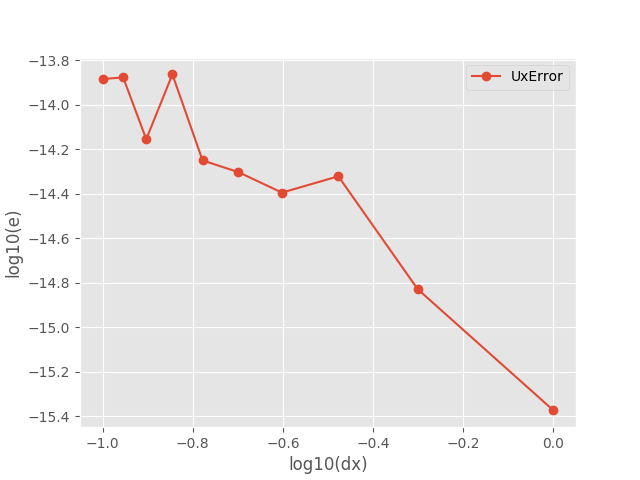
\includegraphics[width=7cm]{chap08/figs/SecondErrorTestSimpleShear.png}
    \caption{Comparação entre solução do grid fino e de diferentes grids grossos.}
\end{figure}

Atestado o bom funcionamento do método dos elementos finitos para solução de problemas com a solução
analítica conhecida, será aplicado agora o método multiescala para verificar o seu correto funcionamento.



Para atestar o bom resultado do método, é importante comparar com soluções que são conhecidas analiticamente. Os testes apresentados são incrementais de forma a testar que todas as opções estão funcionando corretamente.



Primeiro, é apresentado um caso onde as condições de contorno são de Dirichlet Homogêneas. Esse teste tem como domínio $ \Omega = [0, 2] \times [0, 2]$  e como solução a equação apresentada em \ref{eq:solucaoDirichletHomogeneo}.

\begin{equation}\label{eq:solucaoDirichletHomogeneo}
u = 
\begin{bmatrix}
u_x
\\ 
u_y
\end{bmatrix}
=
\begin{bmatrix}
y(-y+2)sen(\pi x))
\\ 
x(-x+2)sen(\pi x))
\end{bmatrix}
\end{equation}

É importante notar que os valores da solução na fronteira do domínio são zero. Pode-se calcular o lado direito referente dessa solução aplicando o operador do problema de elasticidade linear. Fazendo isso, o lado direito encontrado é o mostrado em \ref{eq:ldDiricheletHomogeneo}.


\begin{equation}\label{eq:ldDiricheletHomogeneo}
f(x, y) = 
\left[\begin{matrix}
\begin{split}
\frac{\pi E v x}{v^{2} - 1} \cos{\left (\pi y \right )} - \frac{\pi E v}{v^{2} - 1} \left(- x + 2\right) \cos{\left (\pi y \right )} + \frac{\pi^{2} E y}{v^{2} - 1} \left(- y + 2\right) \sin{\left (\pi x \right )} 
\\
+
\frac{E}{2 v + 2} \left(- \pi x \cos{\left (\pi y \right )} + \pi \left(- x + 2\right) \cos{\left (\pi y \right )} - 2 \sin{\left (\pi x \right )}\right)
\end{split}
\\

\frac{\pi E v y}{v^{2} - 1} \cos{\left (\pi x \right )} - \frac{\pi E v}{v^{2} - 1} \left(- y + 2\right) \cos{\left (\pi x \right )} 
\\
+ \frac{\pi^{2} E x}{v^{2} - 1} \left(- x + 2\right) \sin{\left (\pi y \right )} + \frac{E}{2 v + 2} \left(- \pi y \cos{\left (\pi x \right )} + \pi \left(- y + 2\right) \cos{\left (\pi x \right )} - 2 \sin{\left (\pi y \right )}\right)\end{matrix}\right]
\end{equation}


Assim, o problema descrito em \ref{eq:problemaDirichlet} tem justamente a solução apresentada em \ref{eq:solucaoDirichletHomogeneo}.

\begin{equation} \label{eq:problemaDirichlet}
\begin{matrix}
\nabla \cdot  (C_{dr} : \nabla ^s u) = f(x,y)
\\ 
u_x (x, y)  =  0, \text{em } \partial \Omega
\\ 
u_y (x, y)  =  0, \text{em } \partial \Omega

\end{matrix}
\end{equation}

A figura \ref{fig:DirichletHomogeneo} apresenta a comparação entre a solução de um grid finoe de diferentes tamanhos de elemento grosso. 
O grid fino é constituído de 160 x 160 elementos. Os elementos grossos utilizados tem tamanhos de  2x2, 4x4, 8x8, 16x16 e 32x32 células finas. 
Pode-se observar que quanto maior o engrossamento da malha mais distante da solução analítica é encontrada, até chegar um ponto em que a solução
fica totalmente distorcida. 

\begin{figure}[!htbp]
\label{fig:DirichletHomogeneo}
\centering
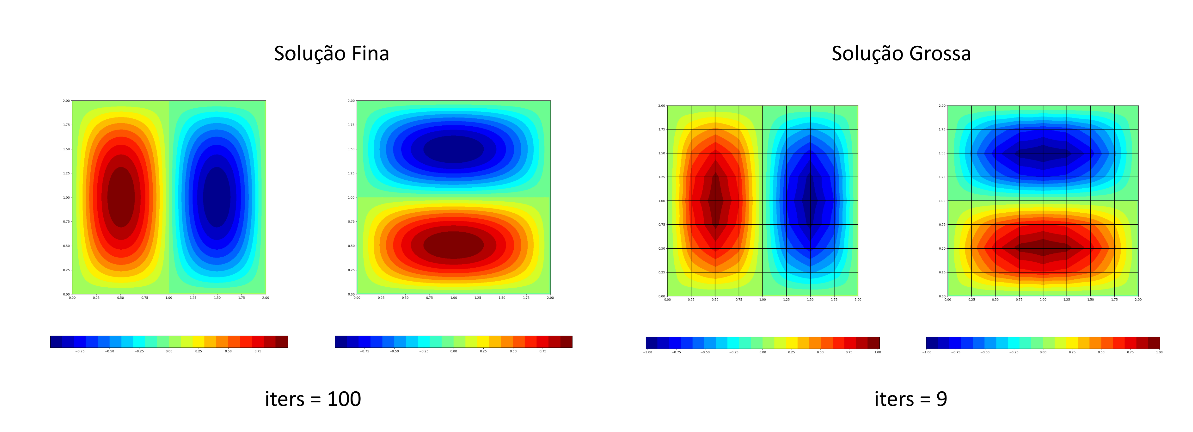
\includegraphics[width=6cm]{chap08/figs/DirichletHomogeneoTemp.png}
\caption{Comparação entre solução do grid fino e de diferentes grids grossos.}
\end{figure}


\begin{figure}[!htbp]
    \label{fig:graficoHomogeneo}
    \centering
    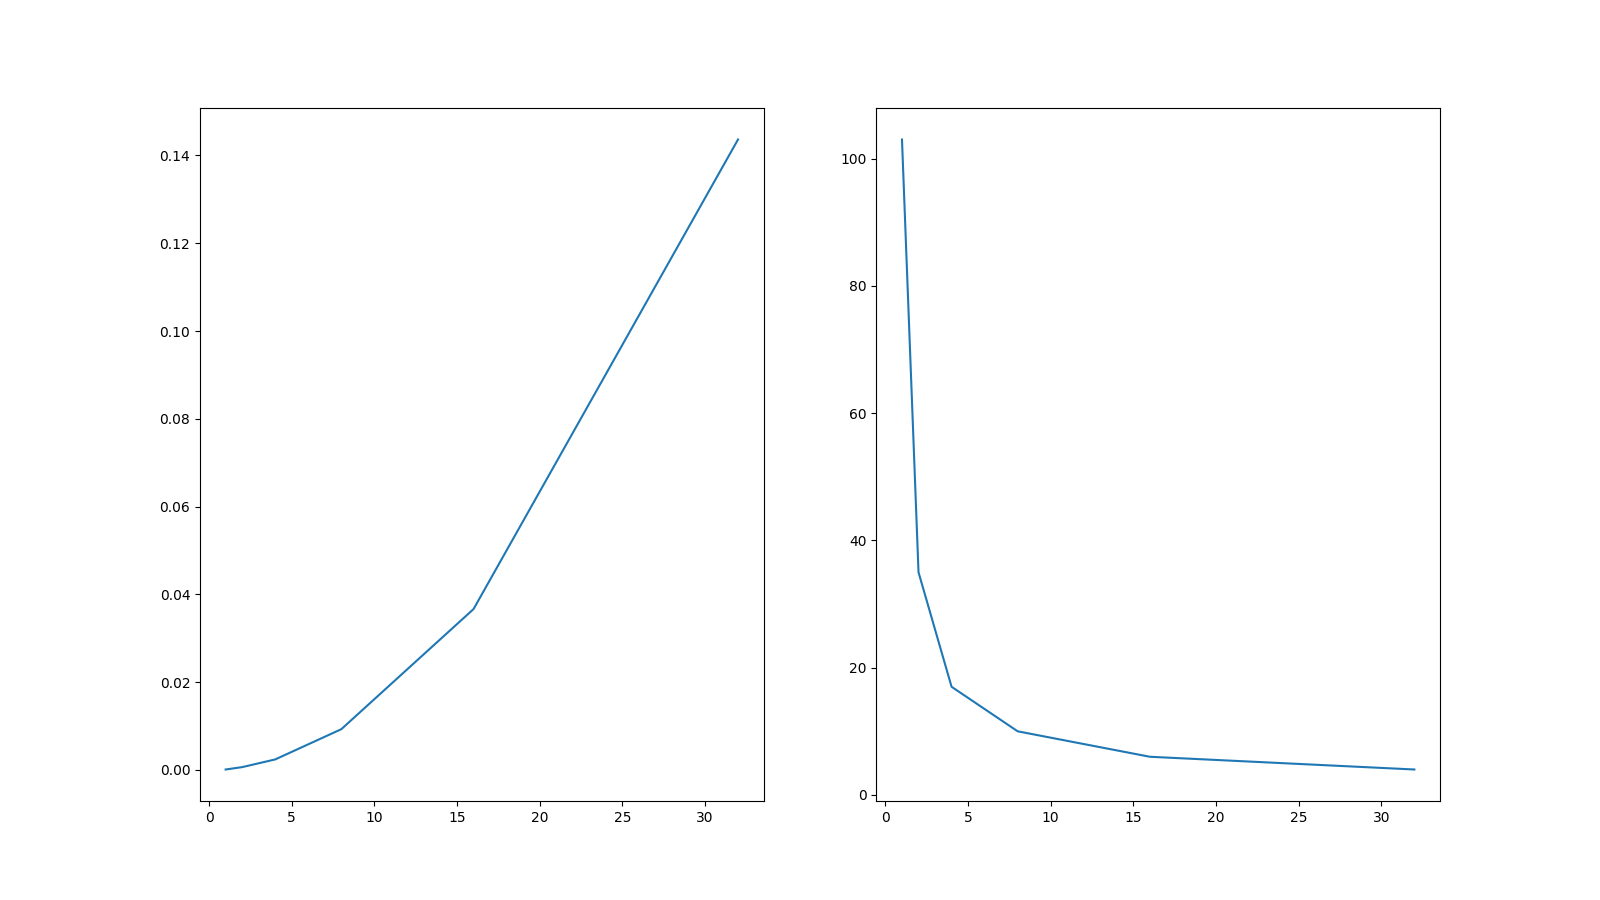
\includegraphics[width=6cm]{chap08/figs/result_analiticos.png}
    \caption{Quantidade de iterações para resolver sistema com gradiente conjugado e ILU(0) e Norma relativa com a solução analítica.}
\end{figure}


\section{Método Multiescala como pré-condicionador}

\subsection{Comparação entre pré-condicionadores aditivos e multiplicativos}

O trabalho \cite{casteletto} apresenta a utilização do pré-condicionador multiescala ($M_{ms}$) em conjunto com o um pré-condicionador ($M_h$) no grid fino de forma multiplicativa. 
Essa combinação visa reduzir os erros de alta frequência através do $M_h$ enquanto os erros de baixa frequencia são eliminados pelo pré-condicionador multiescala. 
O acoplamento multiplicativo tem a desvantagem de precisar de uma multiplicação matriz vetor além da aplicação dos pré-condicionadores
e, portanto, o número de iterações tem que ser reduzido o suficiente para compensar todas essas operações. Um alternativa é aplicação
dos pré-condicionadores de forma aditiva, pois nesse caso não é necessária a multiplicação matriz vetor adicional. Outra vantagem do operador
aditivo é que caso os dois pré-condicionadores sejam simétricos o pré-condicionador conjunto também é simétrico e pode ser utilizado juntamente
com o gradiente conjugado para a solução dos sistemas lineares.


Assim, os casoA e casoB foram utilizados para a comparação do número de iterações entre os dois pré-condicionadores junto 
com o método Bicgstab dado que o pré-condicionador multiplicativo não necessariamente é simétrico. Nesses testes o pré-condicionador $M_h$ utilizado foi o ILU(0).

As tabelas \ref{table:precondcasoAcomp} e \ref{table:precondcasoBcomp} mostram a quantidade de iterações e os respectivos resíduos feita pelos pré-condicionadores aplicados a solução do sistema desses dois reservatórios. 

\begin{table}[]\label{table:precondcasoAcomp}
    \caption{Comparação de pré-condicionador aditivo contra multiplicativo para caso A utilizando como solver linear o método Bicgstab para diferentes níveis de engrossamento do nível grosso.}
    \begin{tabular}{c|c|l|c|l|}

    \cline{2-5}
                                          & \multicolumn{4}{c|}{Pré-condicionador}                                                        \\ \cline{2-5} 
                                          & \multicolumn{2}{c|}{$\preconmult$}               & \multicolumn{2}{c|}{$\preconadd$}                \\ \hline
    \multicolumn{1}{|c|}{Elemento Grosso} & Iterações & \multicolumn{1}{c|}{Resíduo}      & Iterações & \multicolumn{1}{c|}{Resíduo}      \\ \hline
    \multicolumn{1}{|c|}{2x2}             & 7         & \multicolumn{1}{c|}{1.038308e-11} & 9         & \multicolumn{1}{c|}{8.186640e-12} \\ \hline
    \multicolumn{1}{|c|}{5x5}             & 16        & 1.720391e-11                      & 17        & 2.063517e-11                      \\ \hline
    \multicolumn{1}{|c|}{10x10}           & 25        & 1.872316e-11                      & 28        & 5.663356e-12                      \\ \hline
    \multicolumn{1}{|c|}{20x20}           & 38        & 1.643261e-11                      & 38        & 2.842643e-11                      \\ \hline
    \end{tabular}
\end{table}


\begin{table}[]\label{table:precondcasoBcomp}
    \caption{Comparação de pré-condicionador aditivo contra multiplicativo para caso B utilizando como solver linear o método Bicgstab para diferentes níveis de engrossamento do nível grosso.}
    \begin{tabular}{c|c|l|c|l|}
    \cline{2-5}
                                          & \multicolumn{4}{c|}{Pré-condicionador}                                                        \\ \cline{2-5} 
                                          & \multicolumn{2}{c|}{$\preconmult$}               & \multicolumn{2}{c|}{$\preconadd$}                \\ \hline
    \multicolumn{1}{|c|}{Elemento Grosso} & Iterações & \multicolumn{1}{c|}{Resíduo}      & Iterações & \multicolumn{1}{c|}{Resíduo}      \\ \hline
    \multicolumn{1}{|c|}{32x32}           & 86        & \multicolumn{1}{c|}{4.352864e-11} & 80        & \multicolumn{1}{c|}{4.187004e-11} \\ \hline
    \multicolumn{1}{|c|}{64x64}           & 126       & 4.645286e-11                      & 119       & 2.214093e-11                      \\ \hline
    \multicolumn{1}{|c|}{80x80}           & 133       & 4.939883e-11                      & 135       & 3.432757e-11                      \\ \hline
    \end{tabular}
\end{table}


\subsection{Comparação com Multigrid}

Nessa seção, são apresentadas comparações entre o pré-condicionador multiescala e o solver multigrid. Para esse comparação foi utilizado o solver multigrid Pyamg descrito e implementado em \cite{OlSc2018}. Dado a grande quantidade de parâmetros necessários para a configuração dos solver multigrid como: a quantidade de níveis devem ser utilizados, quantidade de relaxações em cada nível, qual o tipo de relaxação será utilizada, dentre outras variáveis, foi utilizado o script solver\_diagnotics.py disponibilizado pela equipe do Pyamg no repositório ( https://github.com/pyamg/pyamg-examples ). Esse script testa sessenta diferentes configurações de solver multigrid e seleciona aquele mais eficiente para o problema proposto.

Os resultados para cada uma das matrizes utilizando mostrou que os solver selecionados como parâmetros: no máximo 15 níveis multigrid, como relaxação utilizavam o "Block Gauss Seidel Sweep" e ciclos V. Sobre a relaxação, o Gauss Seidel Sweep é composta pela aplicação da versão é aplicada nos dois sentidos, atualizando primeiramente o valor  $x_1$  do vetor e depois uma iteração atualizando primeiro o valor  $x_n$. Outra escolha comum para todos os casos, foi a utilização do multigrid como pré-condicionador para o gradiente conjugado.


A figura \ref{fig:reservatorio100x100_1} apresenta o tempo de solução do sistema utilizando o método multiescala e multigrid (Pyamg) como precondicionador para o gradiente conjugado. São apresentados o resíduo ao longo das iterações, o tempo de execução do solver, a quantidade de iterações do solver linear e o tempo da iteração.

\begin{figure}[!htbp]
\label{fig:reservatorio100x100_1}
\centering
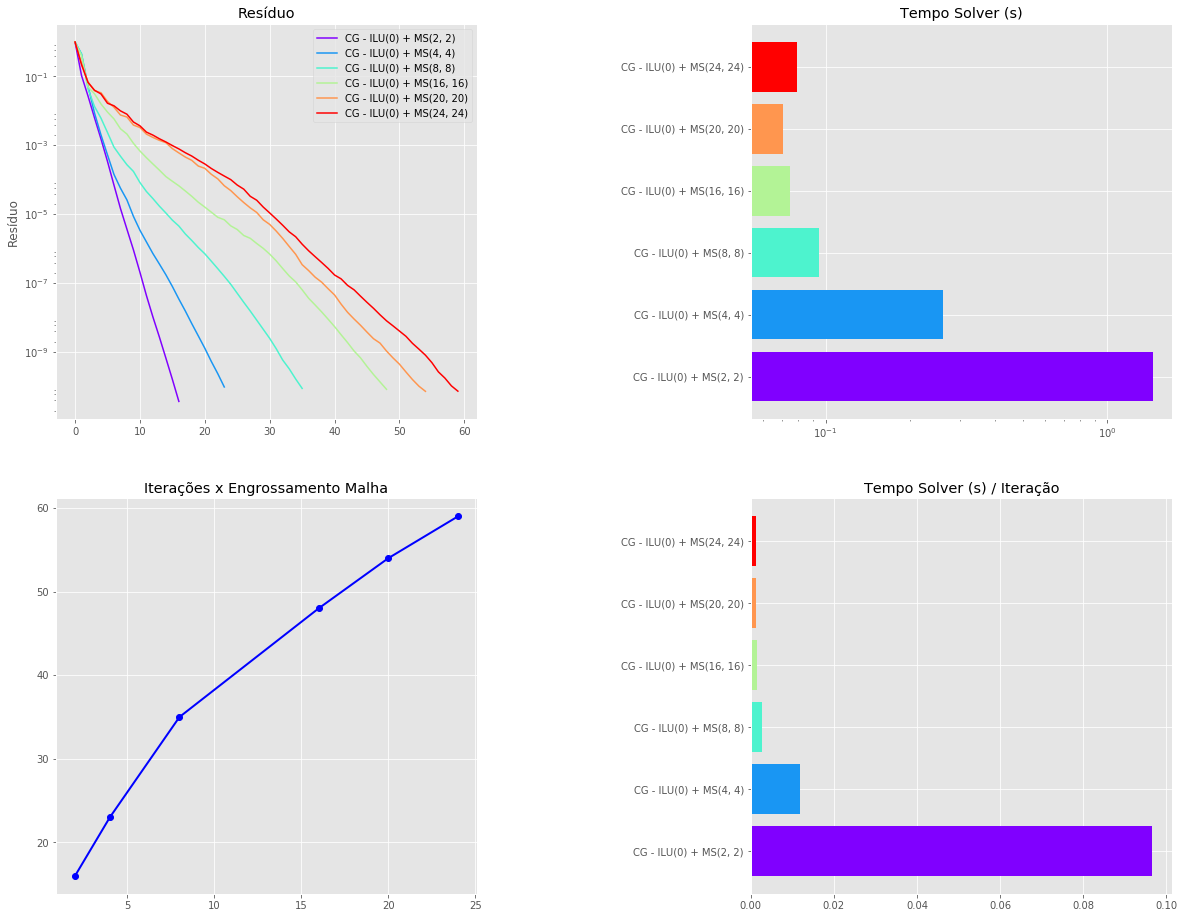
\includegraphics[width=\textwidth]{chap08/figs/reservatorio100x100_1.png}
\caption{Resultados para caso A. Histórico do resíduo relativo ao longo das iterações, tempo do solver em segundos, número de iterações em função do fator de engrossamento da malha e tempo do solver por iteração. }
\end{figure}

Um primeiro ponto a se observar é o aumento do número de iterações a cada vez que se aumenta o fator de engrossamento da malha. Isso ocorre pois a solução do problema grosso se torna cada vez mais distante da solução  original quanto mais a malha perde resolução. Porém, quanto mais grossa a malha, mais rapidamente o sistema linear é resolvido, portanto, existe uma solução de compromisso entre o engrossamento da malha e a quantidade de iterações que serão necessárias para resolver o sistema linear. No caso A, a solução de menor tempo é quando o nível grosso é construído ao se montar elementos grossos utilizando 8x8 elementos finos. 

Na figura \ref{fig:reservatorio100x100_2} é apresentado agora a comparação da solução do sistema utilizando o melhor método multiescala com o gradiente conjugado utilizando como precondicionador o ILU(0), ILU(1) e solver multigrid Pyamg. Pode-se notar que apesar da redução de iterações dos método multiescala e do método multigrid, os pré-condicionadores ILU(0) e ILU(1) são mais eficientes na resolução do sistema. 


\begin{figure}[!htbp]
\label{fig:reservatorio100x100_2}
\centering
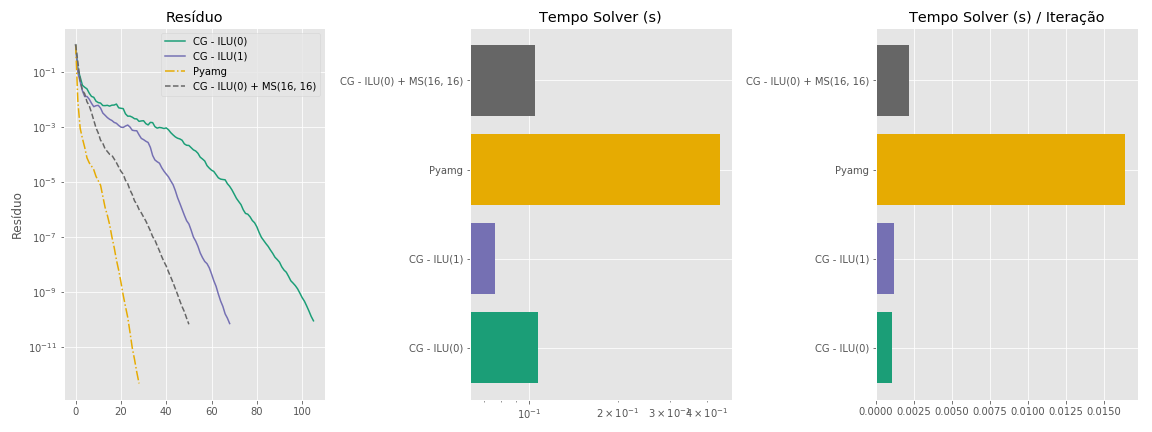
\includegraphics[width=\textwidth]{chap08/figs/reservatorio100x100_2.png}
\caption{Resultados para caso A. Histórico do resíduo relativo ao longo das iterações, tempo do solver em segundos, número de iterações em função do fator de engrossamento da malha e tempo do solver por iteração. }
\end{figure}


As figuras \ref{fig:reservatorio320x320_1} e \ref{fig:reservatorio320x320_2} apresentam os mesmos resultados para o caso B. Nesse caso, o engrossamento multiescala de 20x20 é o que resolve o solver em menor tempo, conseguindo inclusive superar o tempo de solução com o solver pré-condicionador ILU(1).


\begin{figure}[!htbp]
\label{fig:reservatorio320x320_1}
\centering
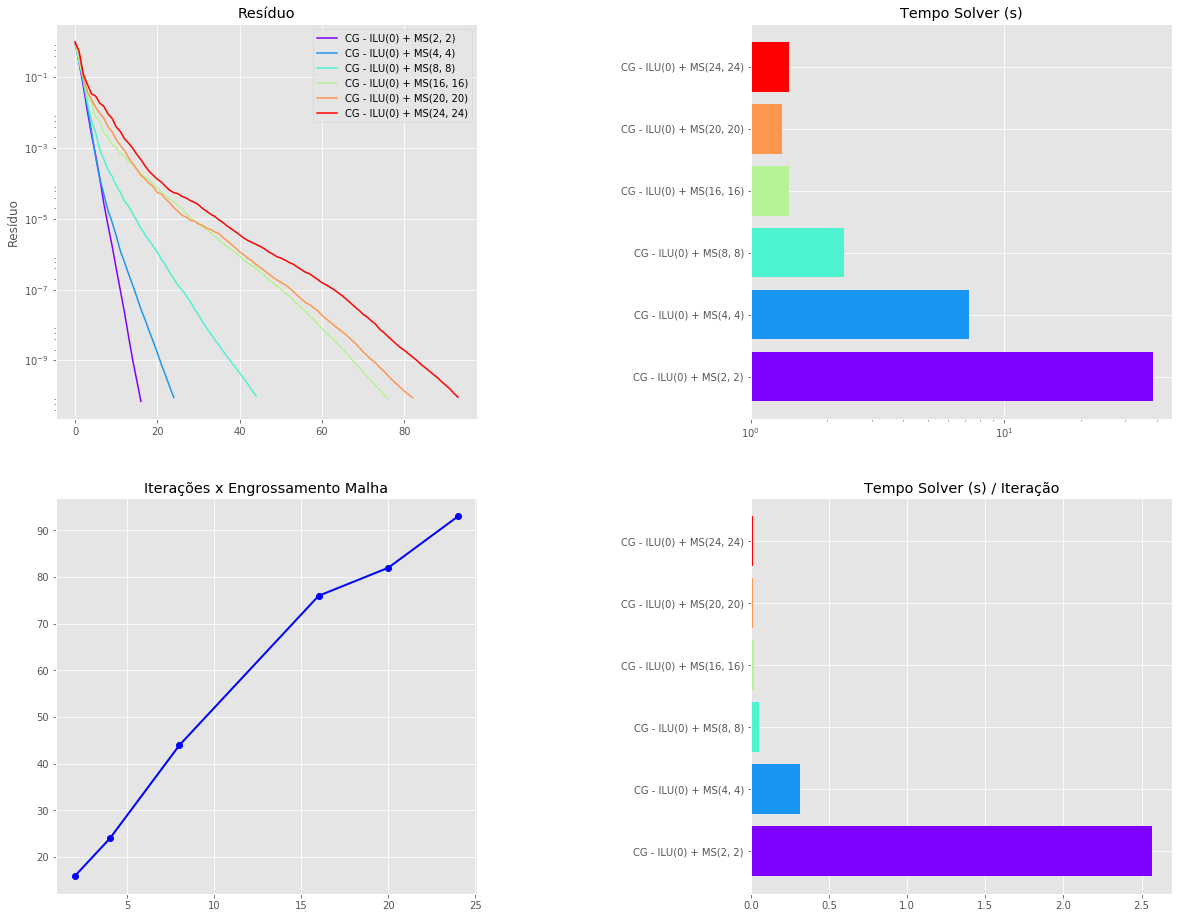
\includegraphics[width=\textwidth]{chap08/figs/reservatorio320x320_1.png}
\caption{Resultados para caso B. Histórico do resíduo relativo ao longo das iterações, tempo do solver em segundos, número de iterações em função do fator de engrossamento da malha e tempo do solver por iteração. }
\end{figure}


\begin{figure}[!htbp]
\label{fig:reservatorio320x320_2}
\centering
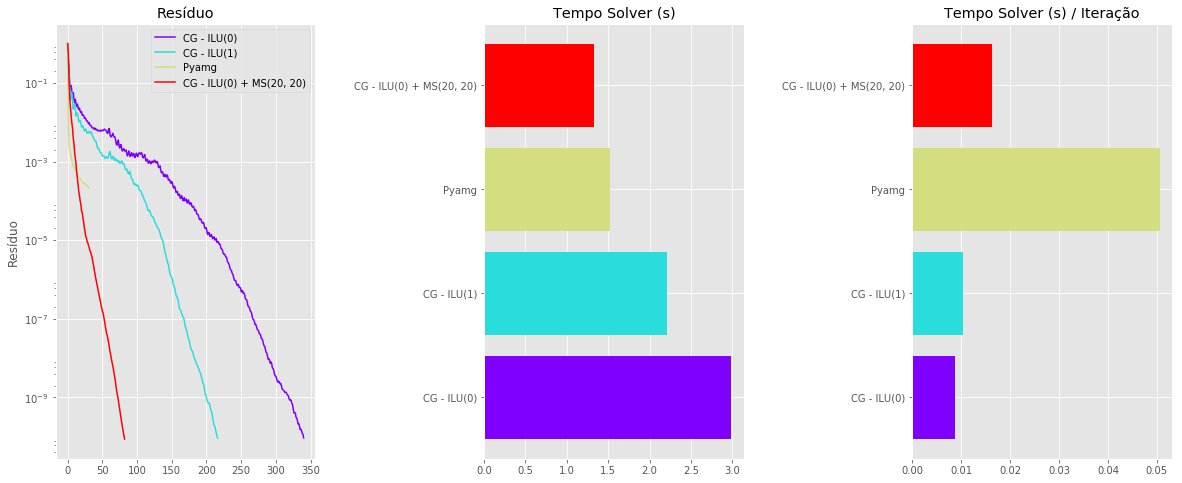
\includegraphics[width=\textwidth]{chap08/figs/reservatorio320x320_2.png}
\caption{Resultados para caso B. Histórico do resíduo relativo ao longo das iterações, tempo do solver em segundos, número de iterações em função do fator de engrossamento da malha e tempo do solver por iteração. }
\end{figure}


A seguir, as figuras \ref{fig:casoC_2}, \ref{fig:casoD_2} e \ref{fig:casoE_2} apresentam os resultados para os casos C, D e E. Em todos os gráficos é mostrado apenas o pré-condicionador multiescala que obteve o melhor desempenho entre os fatores de engrossamento de 2x2, 4x4, 8x8, 16x16, 32x32.


% \begin{figure}[!htbp]
% \label{fig:casoC_1}
% \centering
% 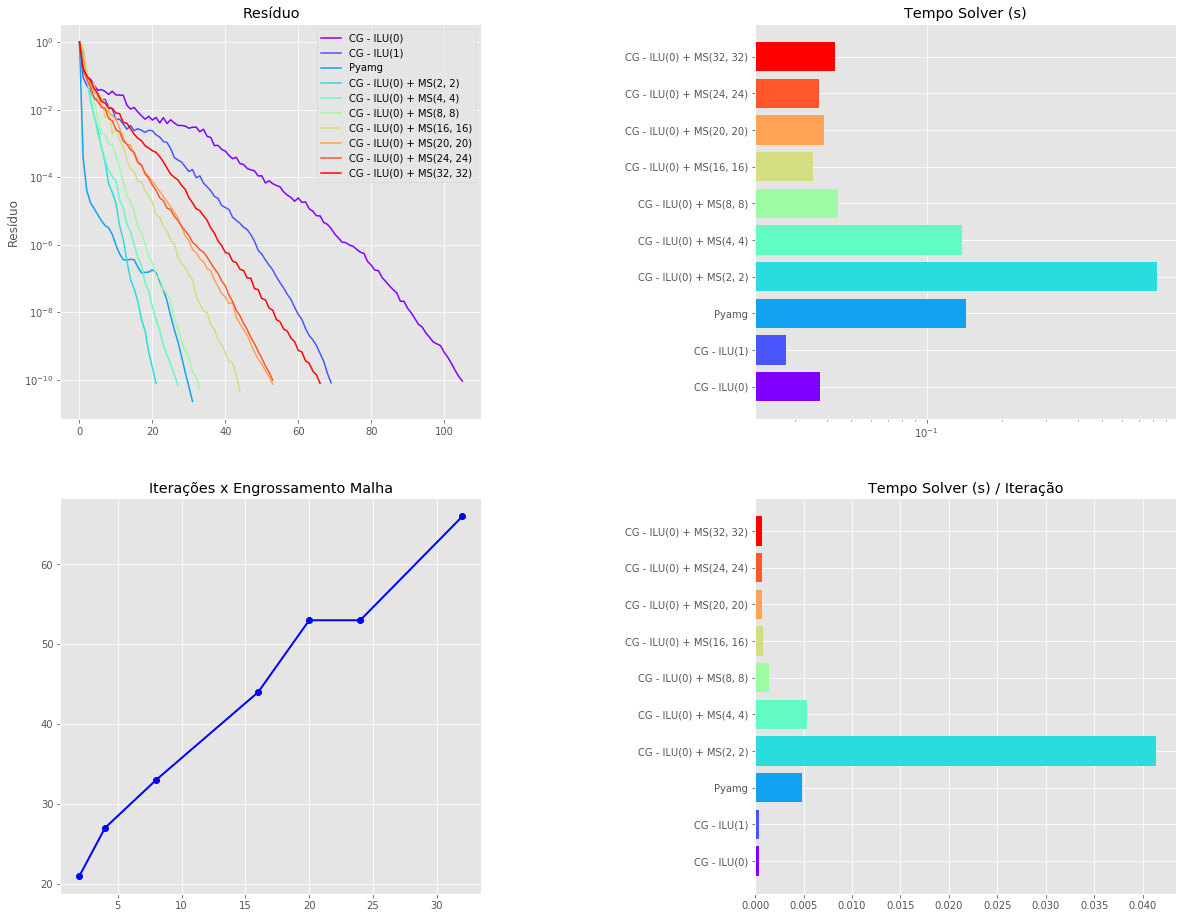
\includegraphics[width=\textwidth]{chap08/figs/casoC_1.png}
% \caption{Resultados para caso C. Histórico do resíduo relativo ao longo das iterações, tempo do solver em segundos, número de iterações em função do fator de engrossamento da malha e tempo do solver por iteração. }
% \end{figure}

\begin{figure}[!htbp]
\label{fig:casoC_2}
\centering
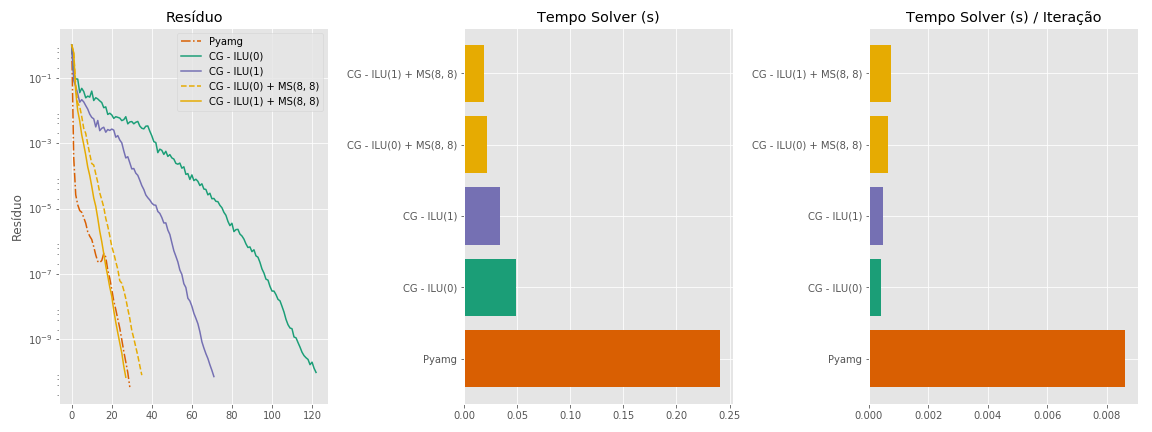
\includegraphics[width=\textwidth]{chap08/figs/casoC_2.png}
\caption{Comparação entre multiescala, multigrid e pré-condicionador ILU para o caso C. Histórico do resíduo relativo ao longo das iterações, tempo do solver em segundos e tempo do solver por iteração. }
\end{figure}



% \begin{figure}[!htbp]
% \label{fig:casoD_1}
% \centering
% 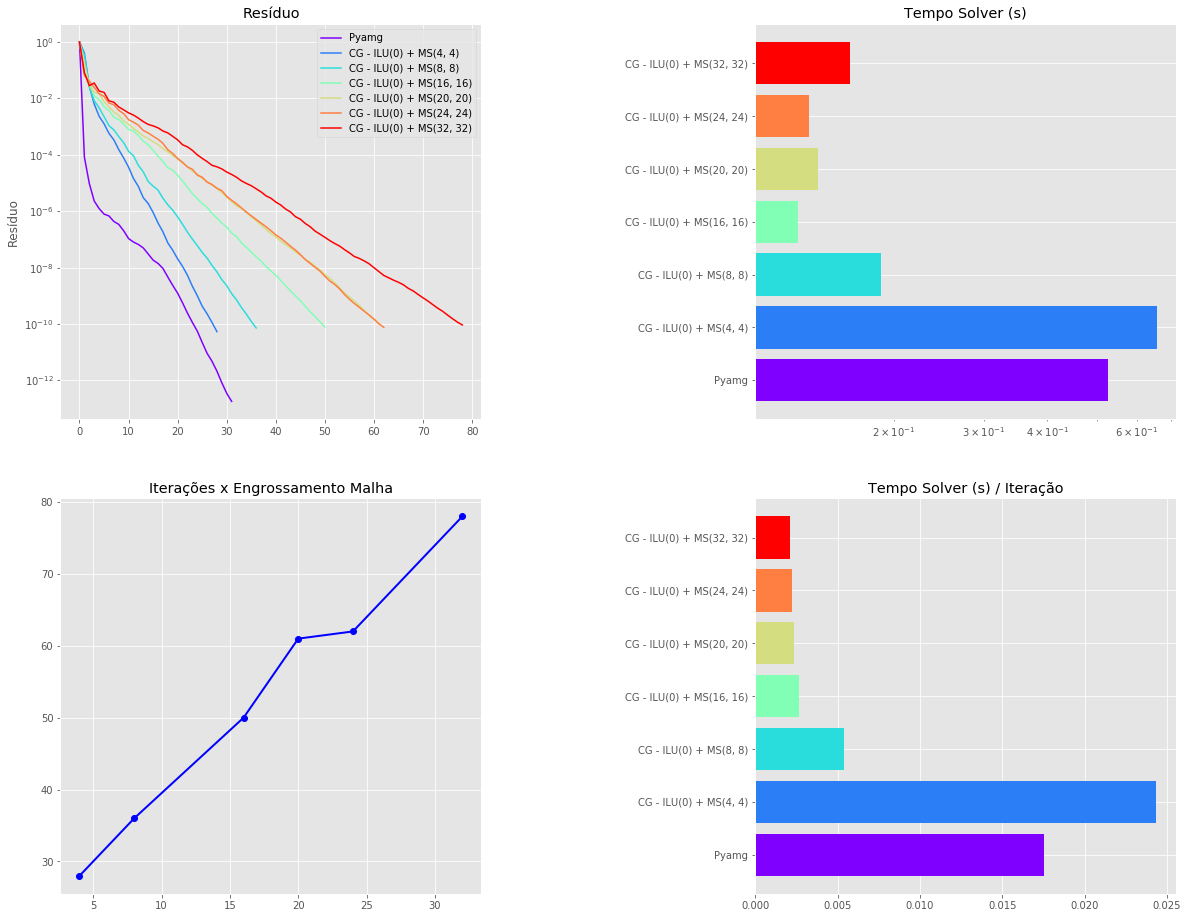
\includegraphics[width=\textwidth]{chap08/figs/casoD_1.png}
% \caption{Resultados para caso D. Histórico do resíduo relativo ao longo das iterações, tempo do solver em segundos, número de iterações em função do fator de engrossamento da malha e tempo do solver por iteração. }
% \end{figure}

\begin{figure}[!htbp]
    \label{fig:casoD_2}
    \centering
    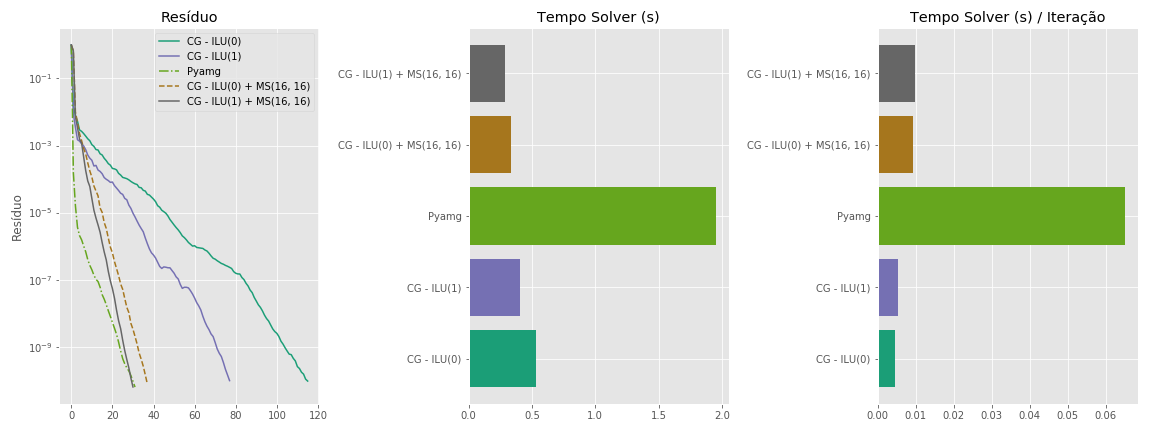
\includegraphics[width=\textwidth]{chap08/figs/casoD_2.png}
    \caption{Comparação entre multiescala, multigrid e pré-condicionador ILU para o caso D. Histórico do resíduo relativo ao longo das iterações, tempo do solver em segundos e tempo do solver por iteração. }
    \end{figure}
    
    % \begin{figure}[!htbp]
    % \label{fig:casoE_1}
    % \centering
    % 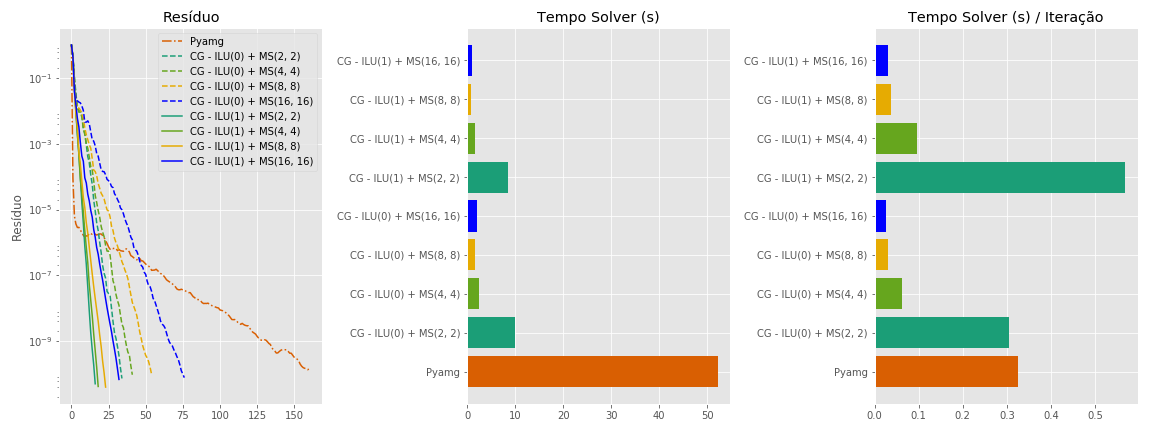
\includegraphics[width=\textwidth]{chap08/figs/casoE_1.png}
    % \caption{Resultados para caso E. Histórico do resíduo relativo ao longo das iterações, tempo do solver em segundos, número de iterações em função do fator de engrossamento da malha e tempo do solver por iteração. }
    % \end{figure}
    
    \begin{figure}[!htbp]
    \label{fig:casoE_2}
    \centering
    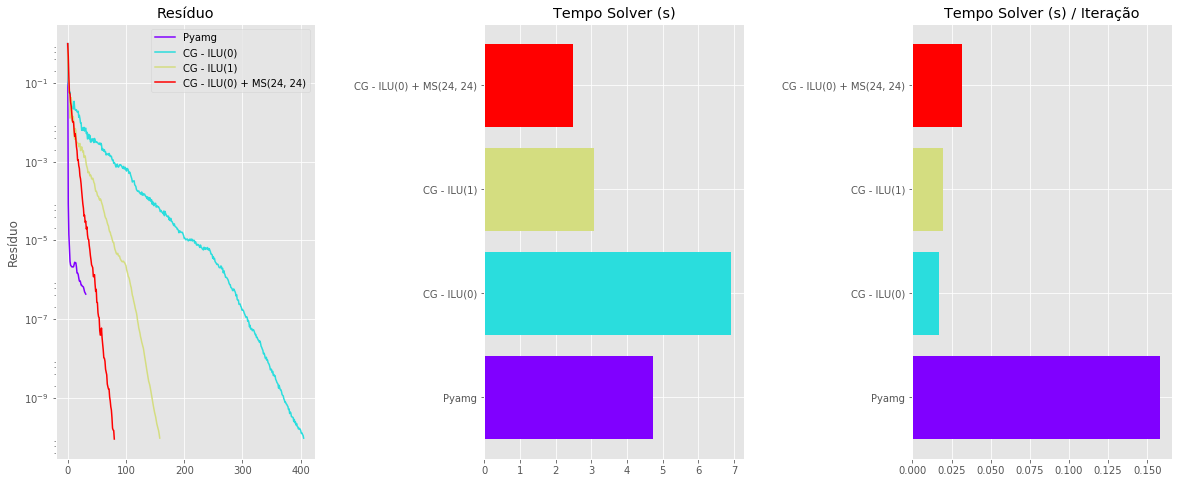
\includegraphics[width=\textwidth]{chap08/figs/casoE_2.png}
    \caption{Comparação entre multiescala, multigrid e pré-condicionador ILU para o caso D. Histórico do resíduo relativo ao longo das iterações, tempo do solver em segundos e tempo do solver por iteração. }
    \end{figure}
